\chapter{Atomi, molecole e ioni}
La chimica studia le proprietà delle sostanze e le loro trasformazioni. Le sostanze sono distinte le une dalle altre dagli elementi che contengono e dato che le proprietà di ciascun elemento sono determinate dagli atomi che lo costituiscono, la chimica è lo studio della materia a livello atomico. Questo fatto fu realizzato da Dalton nel 1807 e segna la nascita della chimica moderna. L'ipotesi atomica di Dalton permise di razionalizzare l'osservazione di sostanze ottenute dalla combinazione di elementi con masse atomiche diverse e predisse una nuova relazione tra gli elementi della tavola periodica, la legge delle proporzioni multiple. Dalton non si limitò a riprendere l'idea di Democrito di atomo; postulò che gli atomi mantengono la loro identità anche quando combinati con altri atomi, ovvero che gli atomi esistono nelle molecole. Una molecola può dunque essere descritta come una collezione di atomi legati tra loro da legami chimici, i quali determinano la struttura della molecola. 
La rivendicazione dell'assunzione di Dalton dovette attendere i risultati degli esperimenti di Rutherford e la sua proposta di atomo nucleare nel 1911. In questo modello, essenzialmente tutta la massa atomica si trova nel nucleo chimicamente stabile. Non solo gran parte della massa ma anche tutta la carica positiva è confinata nel nucleo e questo fatto impartisce l'identità chimica a ciascun atomo. Dagli esperimenti di Rutherford era chiaro che l'atomo era costituito da un nucleo carico positivamente con gli elettroni carichi negativamente disposti in qualche modo intorno ad esso
\paragraph{Spettri atomici.} Quando un gas è attraversato da una scarica elettrica emette luce. La luce può essere generata applicando una forte differenza di potenziale tra gli elettrodi alle estremità di un tubo contenente un gas rarefatto. Un'insegna al neon è un buon esempio di un simile “tubo a scarica”. La cosa interessante è che la luce emessa in questo modo, quando fatta passare attraverso un prisma di diffrazione per separare la luce nelle diverse componenti (frequenze) che la compongono, mostra solo alcune frequenze, al contrario di quanto accade per una sorgente calda che mostra uno spettro continuo. Inoltre, ciascun elemento emette frequenze caratteristiche, ovvero ha uno spettro di emissione caratteristico. In generale, nello spettrogramma sarebbero presenti anche altre righe di emissione che però non sono appartenenti allo spettro del visibile. Da queste osservazioni concludiamo che ogni tipo di atomo, stimolato energeticamente, emette (assorbe) solo certe frequenze caratteristiche: se gli atomi emettono o assorbono solo frequenze “speciali”, gli elettroni responsabili dell'emissione dovranno avere energie speciali.
\paragraph{Effetto fotoelettrico.} Alcuni metalli emettono elettroni quando sono esposti a una sorgente di luce. Questo effetto è noto come effetto fotoelettrico. Alcuni risultati interessanti sono:
\begin{enumerate}
    \item Il numero di elettroni emessi dalla superficie aumenta con l'aumentare dell'intensità della luce incidente ma l'energia cinetica degli elettroni emessi è indipendente dall'intensità.
    \item Non si osserva emissione di elettroni dalla superficie al di sotto di una frequenza minima della luce incidente. Quando gli elettroni sono emessi dalla superficie mostrano una distribuzione di velocità, da zero fino ad un valore massimo. L'energia degli elettroni con la massima velocità aumenta linearmente all'aumentare della frequenza della luce incidente.
\end{enumerate}
Il primo risultato mostra che la luce non può essere descritta in termini ondulatori classici. L'intensità di un'onda è proporzionale al quadrato dell'ampiezza, Al contrario quando le onde elettromagnetiche interagiscono con una certa sostanza solo il numero di elettroni emessi aumenta all'aumentare dell'intensità; l'energia degli elettroni a più alta energia rimane costante. Questo risultato si può spiegare solo se si ammette che l'energia trasportata da un fascio luminoso non è trasmessa nel modo caratteristico di un'onda ma da pacchetti indivisibili (fotoni: quanti di luce), di energia proporzionale alla frequenza della luce stessa. Quindi, l'energia del fotone è direttamente proporzionale alla frequenza della radiazione elettromagnetica secondo la relazione 
\begin{equation}
    E=h\nu.
\end{equation}
Poiché l'elettrone è legato alla superficie del metallo, il fotone deve possedere una quantità minima di energia ovvero una frequenza minima $\nu_0$ sufficiente perché l'elettrone venga rilasciato dal metallo. Quando l'elettrone è emesso dalla superficie a causa di un fotone con frequenza maggiore di questo valore minimo, l'energia in eccesso appare come energia cinetica dell'elettrone emesso, da cui
\begin{equation}
    \overbrace{K_e}^{energia\,cinetica\,e^{-}}=\overbrace{h\nu}^{energia\,fotone}-\overbrace{h\nu_0}^{energia\,minima}.
\end{equation}
Questa equazione stabilisce che l'energia di una radiazione elettromagnetica avente una data frequenza $\nu$ non può essere variata in maniera continua, come nel caso classico, ma viene fornita in “pacchetti” discreti, ognuno dei quali vale $h\nu$. L'energia della radiazione elettromagnetica è quantizzata e un fotone ($h\nu$) corrisponde ad un quanto di energia.

\section{Modello atomico di Bohr}
Bohr considerò un modello planetario in cui l'elettrone orbita intorno al nucleo (un modello compatibile con l'esperimento di Rutherford) e fece le seguenti assunzioni:
\begin{enumerate}
    \item Gli elettroni non emettono radiazione elettromagnetica orbitando intorno al nucleo (come atteso dall'elettromagnetismo classico) ma esistono in stati stazionari ad energia costante.
    \item Gli elettroni possono cambiare la loro energia solo effettuando una transizione da uno stato stazionario ad un altro. Durante questa transizione emettono (o assorbono) una quantità di energia esattamente uguale alla differenza di energia tra i due stati ($\Delta E=E_m-E_0=h\nu$). Questo comportamento produce le righe di assorbimento (o emissione) degli spettri atomici.
\end{enumerate}
Consideriamo una carica negativa $q_1=-e$ che si muove su un'orbita circolare attorno ad una carica positiva $q_2=Ze$, dove $Z$ rappresenta la carica nucleare (uguale a 1 per l'idrogeno). Indicando con $r$ la distanza tra le due cariche la forza di attrazione elettrostatica è data dalla legge di Coulomb
\begin{equation}
    F_C=\frac{-Ze^2}{4\pi\varepsilon_0r^2}.
\end{equation}
Questa forza rappresenta la forza centripeta
\begin{equation}
    F_{CE}=\frac{-m_ev^2}{r},
\end{equation}
da cui, uguagliando si ottiene
\begin{equation}
    m_ev^2=\frac{Ze^2}{4\pi\varepsilon_0r}.
\end{equation}
Integrando la forza di Coulomb rispetto a $r$ si ottiene l'energia potenziale 
\begin{equation}
    V=\int_{\infty}^{r}\frac{-Ze^2}{4\pi\varepsilon_0r^2}dr=\frac{-Ze^2}{4\pi\varepsilon_0r},\qquad V(r)\xrightarrow{r\to\infty}0.
\end{equation}
Quindi, l'energia totale del sistema è 
\begin{equation}
    E_{TOT}=\frac{1}{2}m_ev^2-\frac{Ze^2}{4\pi\varepsilon_0r}=\frac{-Ze^2}{8\pi\varepsilon_0r}.
\end{equation}
Dato che l'energia totale del sistema è negativa significa che il sistema è legato, ovvero è stabile. Per estrarre l'elettrone dal sistema si deve fornire almeno l'energia $E_{TOT}$, infatti questa cambiata di segno corrisponde all'energia di ionizzazione dell'atomo di idrogeno. Nel caso degli atomi ad un solo elettrone, i valori sperimentali dei livelli di energia sono
\begin{equation}
    E_n=\frac{costante}{n^2}.
\end{equation}
Lo stato fondamentale dell'idrogeno corrisponde a $E_1=13.6 eV$, quindi l'espressione generale dell'energie quantizzate è
\begin{equation}
    E_n=\frac{13.6}{n^2}Z.
\end{equation}
Consideriamo ora il momento angolare dell'elettrone
\begin{equation}
    L_e^2={m_evr}^2=m_e\left(m_ev^2\right)r^2=m_e\left(\frac{Ze^2}{4\pi\varepsilon_0}\right)r.
\end{equation}
Combinando questa equazione con quella dell'energia si ottiene la relazione tra $n$ e il raggio delle orbite
\begin{equation}
    r_n=\frac{n^2h^2\varepsilon_0}{\pi Ze^2m_e}.
\end{equation}
Per $n=1$ e $Z=1$ si ha $r_1=a_0=0.529\times10^{-10} m$ il quale viene detto raggio di Bohr, che corrisponde alla distanza elettrone nucleo dell'atomo di idrogeno al suo stato fondamentale. Sostituendo $r_n$ in $E_n$ si ottiene
\begin{equation}
    E_n=-\frac{Z^2}{n^2}\underbrace{\frac{m_ee^4}{8h^2\varepsilon_0^2}}_{K=13.6\,eV},\qquad n\in\mathbb{N}\setminus\{0\},
\end{equation}
dove $n$ è il numero quantico principale e determina l'energia del sistema. Quando $n\to\infty$ e $E\to0$ l'elettrone non risente più della forza elettrostatica ed è libero. La quantità $K$ è l'energia di ionizzazione, ovvero del processo $H\to H^+ + e^-$. 
\paragraph{Spettro dell'idrogeno.} L'energia fornita al gas fa si che molte delle molecole di idrogeno si dissociano in atomi
\begin{equation}
    H_2\to H+H.
\end{equation}
Gli elettroni nelle molecole e negli atomi assorbono energia e sono eccitati a livelli energetici elevati. Quando l'elettrone si trova in un livello energetico superiore al primo (con $n=1$) l'elettrone si dice eccitato (o si trova in uno stato eccitato). La differenza tra due livelli di energia è
\begin{equation}
    \nu=\frac{E_{n'}-E_n}{h},\qquad n'>n.
\end{equation}
Supponendo di considerare tutte le frequenze che appaiono quando un elettrone cade nel livello energetico più basso si ha
\begin{equation}
    \nu=\frac{E_{n'}-E_n}{h}=K/h \left(1-\frac{1}{n^2}\right).
\end{equation}
Nel diagramma, la frequenza risultante da ciascun salto di energia sarà direttamente proporzionale alla lunghezza della freccia. Tanto più le frecce aumentano in lunghezza, tanto più aumenterà la frequenza della luce emessa. Il fatto che l'atomo di idrogeno dia origine a spettri a righe è la prova sperimentale della quantizzazione dei livelli energetici a livello atomico.

\paragraph{Atomi multielettronici.} Il modello di Bohr, anche se prevede correttamente lo spettro dell'atomo di idrogeno, è valido solo per atomi contenenti un solo elettrone, inoltre introduce la quantizzazione delle energie in modo artificioso. Le configurazioni elettroniche degli elementi della tavola periodica verranno dedotte attraverso dati sperimentali forniti dalla spettroscopia fotoelettronica (PES). Nel caso dell'atomo di idrogeno, l'unico elettrone occupa il livello fondamentale , nel caso di atomi multielettronici essi saranno distribuiti su più livelli energetici. I livelli occupati possono essere ottenuti attraverso la meccanica quantistica, ma possono essere ricavati sperimentalmente attraverso la spettroscopia fotoelettronica.
\paragraph{Spettroscopia fotoelettronica (PES).} La spettroscopia fotoelettronica sfrutta l'effetto fotoelettrico.  Quando delle specie atomiche sono esposte ad una luce (fotoni) di energia sufficiente, gli elettroni possono essere emessi da qualunque livello energetico. Quando un campione di un gas contenente un grande numero di atomi di un elemento è bombardato con fotoni di energia sufficiente, ciascun atomo può perdere un elettrone da uno dei suoi livelli energetici. Se viene usata radiazione monocromatica gli elettroni emessi da ciascun livello energetico avranno tutti la stessa energia cinetica.
L'energia in eccesso dell'elettrone è
\begin{equation}
    K_e=h\nu-h\nu_0=h\nu-BE,
\end{equation}
dove $BE$ è l'energia di legame (binding energy) del sistema. Il processo complessivo è descritto in generale da $A\xrightarrow{h\nu}A^+ + e^-$ e dalle equazioni
\begin{equation}
    E_{\left(A\right.)}+h\nu=E_{\left(A^+\right.)}+E_{\left(e^-\right.)}\Rightarrow h\nu=BE+E_{k\left(e^-\right.)}
\end{equation}
La prima equazione mostra la conservazione dell'energia durante la fotoionizzazione. La differenza di energia tra lo stato fondamentale dell'atomo e l'atomo ionizzato rappresenta l'energia di legame dell'elettrone. Poiché ciascun elettrone ha la stessa probabilità di essere emesso, il numero di elettroni emessi sarà proporzionale al numero di elettroni in ciascun livello energetico. La distribuzione degli elettroni negli stati energetici quantizzati prende il nome di configurazione elettronica e si indica con una specifica simbologia. Nel caso dell'idrogeno questa è $1s^1$, in cui il primo numero (1) indica il numero quantico principale ($n$), l'apice il numero di elettroni e la lettera (s) il particolare sotto livello energetico in cui l'elettrone si trova.

\section{Oltre il modello di Bohr}
La descrizione quantistica (l'unica adatta a descrivere l'atomo) comporta il superamento del concetto di orbita e di atomo planetario, descrivendo la distribuzione elettronica in termini probabilistici. Nel caso dell'atomo di Bohr, le orbite elettroniche sono sostituite dal concetto di orbitale. Questo rappresenta la probabilità di trovare l'elettrone in una certa regione di spazio.  Dalla trattazione di Bohr emergeva una sola quantizzazione delle orbite attraverso il numero quantico $n$. L'evidenza sperimentale in accordo con Il risultato della trattazione quanto meccanica indica che ciascun orbitale è caratterizzato da 3 numeri quantici distinti. Il numero quantico principale $n$ è di fatto lo stesso ottenuto dal modello di Bohr. Per un atomo con un solo elettrone è l'unico responsabile dell'energia del livello (orbitale) in cui l'elettrone si trova e delle sue dimensioni dell'orbitale (ovvero della distanza media elettrone-nucleo). Il numero quantico secondario (o di momento angolare) è indicato con $l$ e separa un livello energetico in alcuni sottolivelli. Il numero quantico $l$ può assumere i valori interi da $0$ a $n-1$ e determina l'energia dei sottolivelli  e la forma dell'orbitale (ovvero la distribuzione di densità elettronica) negli atomi con più di un elettrone. In particolare, i sotto livelli $s$, $p$, $d$ corrispondono a valori del numero quantico $l\in\mathbb{N}\setminus\{0\}$. Il terzo numero quantico (o magnetico) $m$ fornisce il numero di orbitali associato a ciascun sottolivello energetico, potendo assumere i valori interi da $-l$ a $+l$. Come emerge dagli spettri PES il numero di elettroni con una data energia è limitato. In particolare abbiamo visto dall'intensità dei picchi degli spettri PES che ci sono due elettroni nei livelli $ns$, sei elettroni nei livelli $np$ e dieci elettroni nei livelli $nd$. Quindi, in ciascun orbitale possono essere allocati al massimo due elettroni.
\begin{figure}[h]
    \centering
    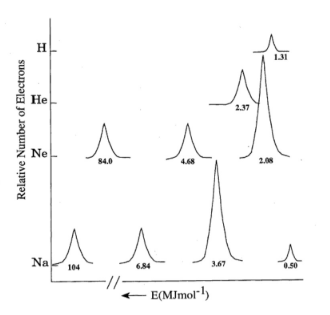
\includegraphics[width=0.5\linewidth,height=0.5\linewidth]{Immagini/Spettro fotoelettronico di H,He,Ne,Na.png}
    \caption{spettro fotoelettronico di H, He, Ne, Na.}
    \label{fig:Spettro fotoelettronico di H,He,Ne,Na}
\end{figure}

L'elettrone è caratterizzato da un momento angolare intrinseco, detto momento angolare di spin di natura quantistica e che non ha analogo classico. Anche questo momento angolare $m_s$ è quantizzato e può assumere solo due valori 
\begin{equation}
    m_s=\pm\frac{1}{2}.
\end{equation}
\begin{axiom}[Principio di esclusione di Pauli]
    Elettroni con lo stesso spin hanno una bassa probabilità di trovarsi vicini e una elevata probabilità di trovarsi lontano gli uni dagli altri, al contrario non ci sono restrizioni per elettroni con spin opposto, che possono trovarsi nella stessa regione di spazio. In altre parole, non possono esistere nello stesso atomo due elettroni con tutti gli stessi numeri quantici.
\end{axiom}
Questo principio giustifica l'evidenza sperimentale secondo la quale in ciascun orbitale ci sono al massimo due elettroni.

\section{Proprietà degli elementi}
Si discutono le proprietà fisiche e chimiche degli elementi in base alla loro configurazione elettronica. La discussione è qualitativa, ma le proprietà che si esaminano possono essere previste in modo accurato attraverso calcoli quantomeccanici.

\subsubsection{Energia di ionizzazione}
 L'energia di ionizzazione ha lo stesso valore assoluto dell'energia di legame ma segno opposto e può essere determinata in modi diversi.
\begin{defn}[Energia di ionizzazione]
    La quantità di energia necessaria per rimuovere un elettrone dall'atomo in
fase gas.
\end{defn} 
Si noti che l'energia necessaria per rimuovere il primo elettrone è detta energia di prima ionizzazione, quella relativa alla rimozione del secondo, energia di seconda ionizzazione, e così via. In generale le energie di ionizzazione di grado superiore al primo sono sempre maggiori, a causa dell'aumento delle forze
elettrostatiche associate allo ione carico.
\begin{figure}[h]
    \centering
    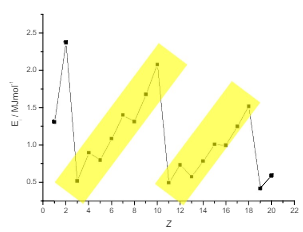
\includegraphics[width=0.5\linewidth]{Immagini/Diagramma energie di ionizzazione.png}
    \caption{diagramma delle energie di ionizzazione.}
    \label{fig:Diagramma energie di ionizzazione}
\end{figure}

L'esame del diagramma rivela un'evidente regolarità. Tra gli elementi Li e Ne c'è un graduale aumento dell'energia di ionizzazione $E_i$ all'aumentare di $Z$, con due piccole depressioni in corrispondenza degli elementi boro e ossigeno. Questo andamento è riprodotto anche per gli elementi dal sodio all'argon. L'effetto dell'aumento dell'energia di ionizzazione è correlato all'incremento delle forze di attrazione del nucleo man mano che aumenta il numero di protoni. Le irregolarità osservate per B e O meritano qualche osservazione. Poiché il quinto elettrone del boro entra in un orbitale $2p$ la cui densità elettronica si estende più lontano dal nucleo rispetto a quella degli elettroni $2s$, la sua energia di ionizzazione è più piccola di quella degli elettroni $2s^2$ del berillio. Nel caso del quarto elettrone $p$ dell'ossigeno si osserva un calo simile di $E_i$. In questo caso il nuovo elettrone condivide un orbitale con uno dei precedenti elettroni $2p$. L'energia di interazione, cioè la repulsione elettrostatica tra due elettroni nella stessa regione di spazio, rende più facile la rimozione dell'elettrone, diminuendo l'energia di ionizzazione. All'inizio di ogni nuovo periodo si osserva una significativa diminuzione dell'energia di ionizzazione, consistente con il fatto che all'inizio di ogni periodo aumenta il numero quantico principale $n$ così che il nuovo elettrone $s$ ha un'energia di legame molto inferiore. In generale le energie di ionizzazione aumentano muovendosi da sinistra a destra nella tavola periodica (variazione più significativa) e diminuiscono muovendosi dall'alto verso il basso in un gruppo (variazione meno significativa).
\subsubsection{Affinità elettronica}
In alcuni casi favorevoli è possibile determinare l'energia rilasciata quando un elettrone è aggiunto all'atomo neutro formando uno ione negativo. 
\begin{defn}[Affinità elettronica]
    La quantità di energia liberata da un atomo quando un elettrone viene aggiunto alla sua configurazione, quando questa si trova in stato neutro isolato in forma gassosa, per formare uno ione negativo
\end{defn}
Quest'energia corrisponde all'energia necessaria per liberare un elettrone dallo ione negativo secondo $A_{\left(g\right.)}^{-}\to A_{\left(g\right.)} + e^-$. La convenzione è che se è richiesta energia per rimuovere l'elettrone dallo ione negativo, l'affinità elettronica è positiva. A prima vista può sembrare sorprendente che un atomo neutro possa attrarre un elettrone extra. Consideriamo però la configurazione di valenza di un elemento del settimo gruppo, gli alogeni, $ns^2np^5$. A causa della schermatura incompleta da parte degli altri elettroni del guscio di valenza, la vacanza presente, eserciterà una forza attrattiva sufficientemente elevata da legare un elettrone libero all'atomo. 

Le affinità elettroniche dei gas nobili saranno in effetti zero, perché, nonostante la carica nucleare effettiva sia massima, l'extra elettrone dovrà entrare in un orbitale caratterizzato da numero quantico superiore, dove risentirà di una debole carica effettiva a causa dell'effetto di schermo esercitato dagli elettroni nei gusci interni. Gli elementi alla sinistra della tavola periodica hanno un'affinità elettronica bassa e in alcuni casi nulla. L'affinità elettronica aumenta muovendosi verso destra lungo un periodo raggiungendo un massimo nel caso degli alogeni. Questo andamento riflette in maniera diretta la variazione della carica nucleare effettiva. L'affinità elettronica diminuisce quindi scendendo lungo un gruppo nella tavola periodica. 

In questo modo l'affinità elettronica è simile all'energia di ionizzazione, con la differenza che, mentre l'energia di ionizzazione è sempre positiva (ovvero è sempre necessario spendere energia per separare l'elettrone dal nucleo nell'atomo neutro), l'affinità elettronica può avere valori nulli (o anche valori negativi non direttamente misurabili sperimentalmente), indicanti il fatto che la specie ionica carica negativamente non è stabile in fase gas.
\subsubsection{Raggi atomici e raggi ionici}
l diametro di un atomo è una quantità difficile da definire in modo preciso, poiché la distribuzione di densità elettronica va a zero a distanze molto grandi dal nucleo. Tuttavia esiste un limite alla vicinanza con cui due atomi possono essere spinti. Le dimensioni atomiche tendenzialmente diminuiscono all'aumentare del numero atomico, man mano che aumenta il numero di elettroni all'interno di un guscio con numero quantico principale $n$. 
\begin{figure}[h]
    \centering
    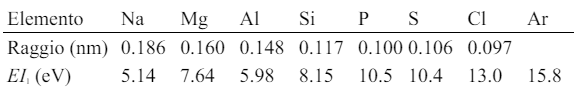
\includegraphics[width=0.7\linewidth]{Immagini/Raggi atomici e energie di prima ionizzazoine III gruppo.png}
    \caption{raggi atomici e energie di prima ionizzazione (III gruppo).}
    \label{fig:Raggi atomici e energie di prima ionizzazoine III gruppo}
\end{figure}
Dalla tabella si osserva come l'energia di ionizzazione aumenti al diminuire del raggio atomico. Questo fatto trova la sua spiegazione attraverso il concetto di carica nucleare efficace. Il campo elettrico e quindi la forza di attrazione esercitata dal nucleo sull'elettrone nel guscio di valenza più esterno è ridotto a causa degli effetti di schermo esercitato dagli altri elettroni presenti nell'atomo. Gli elettroni nel guscio di valenza più esterno esercitano un effetto di schermo molto ridotto, quindi più alto è il rapporto tra elettroni esterni ed elettroni interni, maggiore sarà la carica nucleare efficace sentita da un elettrone nel guscio più esterno. Il numero di elettroni esterni aumenta lungo il periodo, ma il numero di elettroni nel guscio interno rimane costante. Quindi la carica nucleare effettiva aumenta da un valore minimo per il sodio, in cui il rapporto tra elettroni esterni ed interni è $1:10$, fino a un valore massimo per l'argon, dove lo stesso rapporto è $8:10$. Quindi, il raggio atomico diminuisce gradualmente dal momento che gli elettroni del guscio più esterno sono via via più fortemente attratti dalla carica nucleare effettiva. 
\begin{figure}[ht]
    \centering
    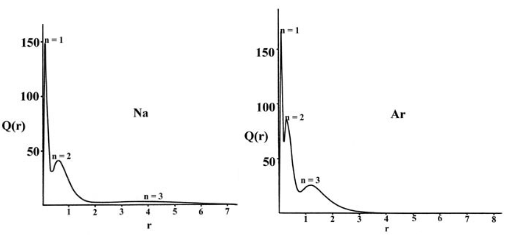
\includegraphics[width=0.7\linewidth]{Immagini/Funzione Q(r).png}
    \caption{funzione $Q(r)$ per Na e Ar.}
    \label{fig:Funzione Q(r)}
\end{figure}

Queste caratteristiche della distribuzione della densità elettronica sono chiaramente evidenti in un grafico della funzione di distribuzione radiale, $Q(r)$, che descrive il numero di cariche elettroniche in una regione di spazio localizzata tra due sfere concentriche di raggio $r$ e $r + dr$. L'effetto più vistoso nella differenza delle cariche effettive di argon e sodio è evidenziato dalla densità elettronica nel guscio di valenza $n=3$. Nel sodio questo guscio è molto diffuso, dal momento che ci sono dieci cariche elettroniche interne che schermano undici cariche nucleari. Nell'argon, dove ci sono dieci elettroni interni che schermano diciotto cariche nucleari, il guscio di valenza è molto più contratto e ha il suo massimo a circa un terzo della corrispondente distanza nel sodio.
\begin{obs}
    Nella tabella si nota un'eccezione all'andamento su descritto nel caso del fosforo. Questo ha un raggio atomico leggermente inferiore a quello dello zolfo che lo segue e corrispondentemente un'energia di prima ionizzazione leggermente superiore. La configurazione degli elettroni di valenza del fosforo è $3s^23p^3$. Ciascuno degli orbitali $p$ contiene un singolo elettrone e secondo la regola di Hund tutti saranno caratterizzati dallo stesso numero di spin. Elettroni con lo stesso spin hanno repulsioni elettrone-elettrone minori di quelle associate a elettroni con spin accoppiati. Per tanto maggiore è il numero di elettroni con lo stesso spin in un atomo, minore sarà l'energia media di repulsione tra gli elettroni. Tre è il numero massimo di elettroni possibili nel periodo caratterizzato da n=3 e corrisponde al semiriempimento degli orbitali p. L'effetto di stabilizzazione associato alla diminuzione dell'energia di repulsione tra gli elettroni è comparabile all'effetto ottenuto aumentando la carica nucleare effettiva di circa un'unità. Questo può essere visto confrontando il fosforo con lo zolfo. Lo zolfo ha una carica nucleare maggiore ma l'elettrone in più deve accoppiarsi con spin antiparallelo, con uno degli elettroni negli orbitali p. Il numero di elettroni con spin paralleli è quindi ridotto a due, l'energia media di repulsione aumenta e lo zolfo ha dimensioni leggermente maggiori di quelle del fosforo che lo precede e energia di ionizzazione leggermente inferiore. 
\end{obs}

Il valore medio della distanza elettrone nucleo aumenta all'aumentare del valore del numero quantico principale. L'aumento nelle dimensioni atomiche scendendo lungo un gruppo è quindi facilmente comprensibile. In particolare passando dall'ultimo membro del periodo n (guscio chiuso, gas nobile) all'elemento successivo (metallo alcalino) ci sarà una diminuzione repentina della carica effettiva dal momento che il numero di elettroni interni aumenta di otto unità. Inoltre il nuovo elettrone dovrà, secondo il principio di Pauli, entrare in un orbitale caratterizzato da numero quantico n superiore. Tutto ciò fa si che gli elementi del primo gruppo abbiano dimensioni maggiori e energie di ionizzazione più basse dei gas nobili che li precedono. In generale, la diminuzione della carica nucleare effettiva e l'aumento del numero quantico principale scendendo lungo un gruppo, comporta una diminuzione
dell'energia di ionizzazione.
\subsubsection{Energia di configurazione e elettronegatività}
La reattività chimica e il legame chimico dipendono in modo cruciale dall'energia di legame degli elettroni di valenza ovvero dalla forza di attrazione esercitata da ciascun “guscio atomico”. Questa forza può essere misurata (approssimativamente) dall'energia media degli elettroni di valenza, ovvero dall'energia di una data configurazione elettronica di valenza.

Allen ha suggerito che l'energia media di una data configurazione elettronica di valenza può essere ottenuta da
\begin{equation}
    CE=\chi=\frac{aE_s+bE_p}{a+b},
\end{equation}
dove $a$ e $b$ rappresentano il numero di elettroni $s$ e $p$, e $E_s$ ed $E_p$ rapprensentano le corrispondenti energie di ionizzazione. Questa equazione fornisce con buona approssimazione la forza di attrazione esercitata
da ciascun “guscio atomico”, che coincide con la definizione di elettronegatività.
\begin{defn}[elettronegatività di Pauling]
    La capacità di un atomo in una molecola di attrarre gli elettroni di
legame e derivata dalle energie di legame.
\end{defn}
Dalla definizione fornita
è evidente che l'elettronegatività è una proprietà periodica e riflette direttamente l'energia associata ai
sottolivelli elettronici (orbitali) in via di riempimento lungo un periodo. La tavola periodica è caratterizzata
da due dimensioni, la carica nucleare, $Z$, che aumenta lungo un periodo e il numero quantico principale $n$,
che aumenta scendendo lungo un gruppo. L'elettronegatività fornisce una terza dimensione che ha le unità
di un'energia e descrive la variazione energetica man mano che i sottolivelli associati a ciascun periodo (gusci
elettronici) vengono riempiti.
\begin{obs}
    Scendendo lungo un gruppo l'elettronegatività diminuisce per le stesse ragioni
descritte nei paragrafi precedenti relativamente alle dimensioni atomiche e energie di ionizzazione. Gli
elementi che tendono a dare origine a ioni positivi (metalli) sono caratterizzati da valori di elettronegatività
relativamente piccoli rispetto ad elementi indicati come non metalli.
\end{obs}